\subsection{Objective 1: Heading for this chapter}
\label{objective1}
A brief bit of introduction to this chapter (1-2 paragraphs)

\subsubsection{Research Plan}
 What methods do you have planned for this chapter? Here you should describe what your concrete plans are for addressing this objective. You also might want to include a figure in this portion, such as Fig. \ref{fig:colonization_hypothesis}.
 
 %% FIGURE %%
\begin{figure}[tb]
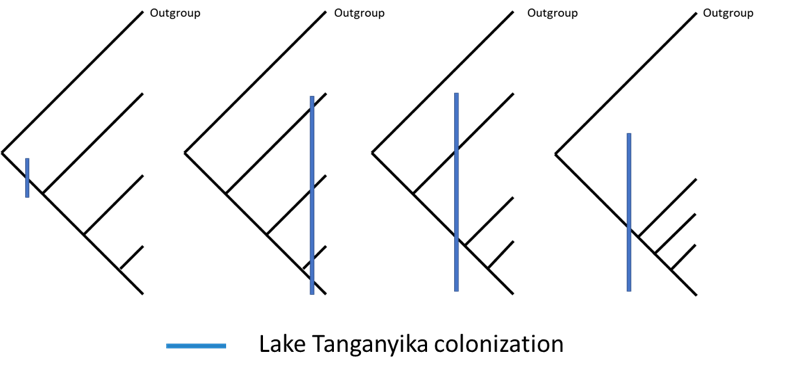
\includegraphics[width=\textwidth]
{figures/colonization_hypothesis.png}\caption{\label{fig:colonization_hypothesis} Hypotheses to test about the colonization of Lake Tanganyika (LT) by Lates fishes and their diversification times. (A) A common ancestor colonized LT and each of the species split off from the others in succession; (B) the four species diversified prior to colonizing LT; (C) two different ancestors colonized LT, followed by diversification of one of those species; (D) a common ancestor colonized the lake, and the four species split at roughly the same time, forming a true radiation.}
\end{figure}
%%%%
 
 \textsc{Method A ---} You can use subheadings to separate out different things you'll be doing for this chapter. Perhaps your subsections can be "sampling," "data generation," and "analysis" (these are what mine are!).
 
 \textsc{Method B ---} And here's a second subsection of things that I'll be doing.
 
\subsubsection{Specific Questions}
\begin{enumerate}
    \item \textbf{Question \#1}
    
    A bit of explanation about this question, if necessary, and perhaps what your hypothesis is for this question.
    
    \item \textbf{Question \#2}
    
    Explanation for this question.
    
\end{enumerate}

\subsubsection{Expected Outcomes}
What things do you anticipate coming from this chapter?